%\VignetteIndexEntry{CloneFinder}
%\VignetteKeywords{SNP,Copy Number,clone,subclone}
%\VignetteDepends{stats}
%\VignettePackage{CloneFinder}
\documentclass{article}

\usepackage{hyperref}

\newcommand{\Rfunction}[1]{{\texttt{#1}}}
\newcommand{\Robject}[1]{{\texttt{#1}}}
\newcommand{\Rclass}[1]{{\texttt{#1}}}
\newcommand{\Rpackage}[1]{{\textit{#1}}}

\title{Inferring Clonal Structure From SNP Copy Number Data}
\author{Kevin R. Coombes and Mark Zucker}

\usepackage{Sweave}
\begin{document}
\input{cloneFinder-concordance}

\maketitle
\tableofcontents

\section{Introduction}


\section{Getting Started}

We start by loading the package into the current R session.
\begin{Schunk}
\begin{Sinput}
> library(CloneFinder)
\end{Sinput}
\end{Schunk}

\section{Structure of the Algorithm}

\subsection{Compartments}
We introduce the term \textit{compartment} to describe a pure
(undiluted, homogeneous) copy number state.  For modeling purposes, we
assume that there is a fixed number of pure compartments.  In
particular, we do not model high amplifications in copy number, mainly
because they are simply indistinguishable in SNP copy number data.

We consider the following comparments:
\begin{itemize}
\item Most segments of the genome appear in two different (i.e.,
  heterozygous) copies.  In this state, we expect the true log R ratio
  ($LRR$) to equal zero and the true B allele frequency ($BAF$) to
  equal one-half.
\item Some segments contain two identical (homozygous) copies of the
  genomic material, either through inheritance (identical by descent)
  or because of a somatic loss of heterozygosity (LOH).  In this case,
  the true $LRR = 0$ and the true $BAF = 0$.
\item Another compartment arises when all cells in the sample being
  measured have lost one copy of a genomic segment.  In this case,
  the true $LRR = \log(1/2)$ and the true $BAF = 0$.
\item Similarly, it is possible for all cells in the sample to acquire a
  gain of the same genomic segment.  In this case, the true
  $LRR=\log(3/2)$ and the true $BAF = 1/3$.
\item A gain of two copies of the same piece of a chromosome has true
  $LRR=\log(2)$ and true $BAF = 1/4$.   (For modeling purpoises, we
  ignore the tetraploidy case when both parental chromosomes are
  duplicated, leading to $LRR=\log(2)$ and $BAF = 1/2$.)  We also
  ignore higher copy number gains. 
\item The case when both copies of a genomic segment is problematic,
  since the true $LRR = \log(0) = -\infty$ and the true $BAF = 0/0$ is
  undefined.
\end{itemize}

\paragraph{Code Example}
A compartment is modeled in the \texttt{CloneFinder} package by the
\texttt{CompartmentModel} class, which is implemented as:
\begin{Schunk}
\begin{Sinput}
> showClass("CompartmentModel")
\end{Sinput}
\begin{Soutput}
Class "CompartmentModel" [package "CloneFinder"]

Slots:
                                          
Name:      markers pureCenters      sigma0
Class:     numeric  data.frame     numeric

Known Subclasses: "Tumor"
\end{Soutput}
\end{Schunk}

In this preliminary implementation, instead of using actual
$(LRR,BAF)$ pairs, we instead simulate and model the data as though it
comes from a pair of independent normal distributions.  For example,
\begin{Schunk}
\begin{Sinput}
> set.seed(2726642) # for reproducible examples
> nSeg <-  1000     # number of segments supposedly found by CBS
> markers <- round(runif(nSeg, 25, 1000))  # numbers of markers
> # set 'known' centers for the pure compartments
> xy <- data.frame(x = c(0.2, 0.7, 0.8, 0.1, 0.4),
+                  y = c(0.2, 0.3, 0.5, 0.9, 0.7))
> # build the model. sigma0 = std dev at one marker
> baseModel <- CompartmentModel(markers, xy, sigma0=0.25)
> rm(nSeg, xy)
\end{Sinput}
\end{Schunk}

Before we can show you how the modeling works, we have to simulate
data from a tumor.
\begin{Schunk}
\begin{Sinput}
> wts <- rev(5^(1:5))
> wts <- wts/sum(wts)  # prevalence of differnt compartments
> fracs <- c(5, 3, 1)  # relative frequency of subclones
> # length of 'fracs' is the number of clones
> # now simulate a tumor;
> tumor <- Tumor(baseModel, fracs, wts)
> rm(wts, fracs, markers, baseModel)
> class(tumor)
\end{Sinput}
\begin{Soutput}
[1] "Tumor"
attr(,"package")
[1] "CloneFinder"
\end{Soutput}
\end{Schunk}
Objects of the \texttt{Tumor} class are basically multivariate
distributions; you have to make another function call to
sample/simulate data from them.
\begin{Schunk}
\begin{Sinput}
> simdata <- generateData(tumor)
\end{Sinput}
\end{Schunk}
\begin{figure}
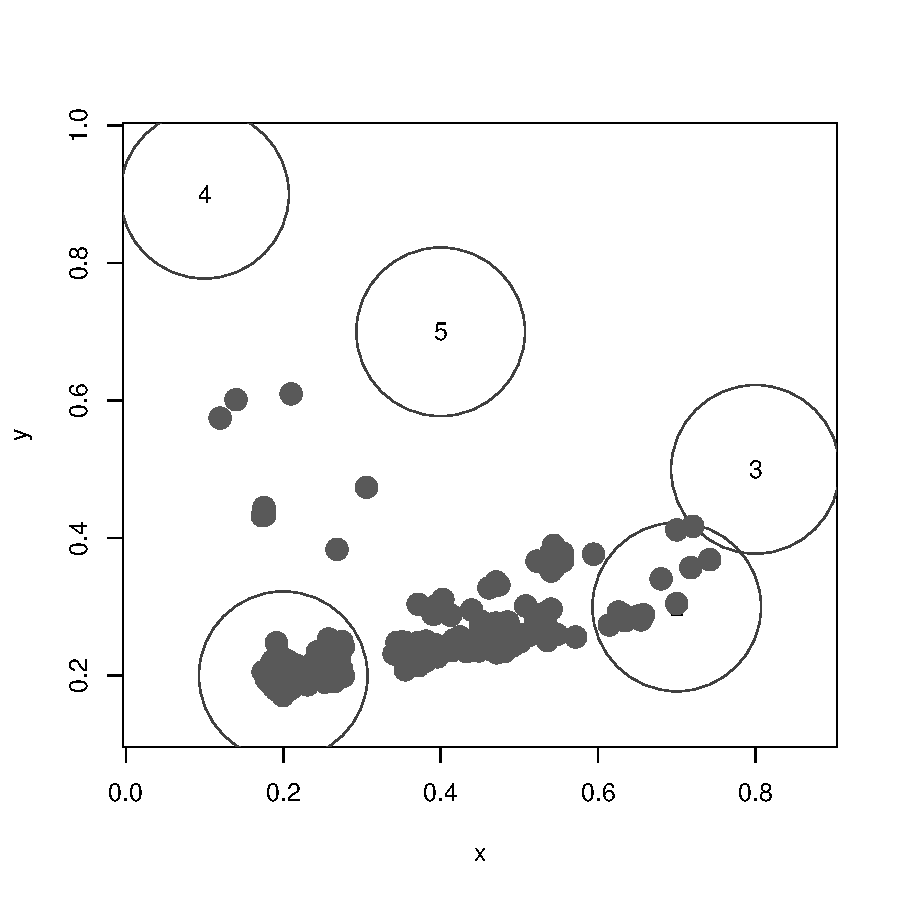
\includegraphics{cloneFinder-006}
\caption{Sized scatter plot of simulated data.}
\label{sizeplot}
\end{figure}

\subsection{Segment-Level Modeling}
After the SNP copy number data has been segmented (typically by
applying something like the circular binary segmentaion algorithm
implemented in the \texttt{DNAcopy} R package), we model the data as
arising from a mixture (in terms of cells in the biological sample) of
the pure compartments.  We use the following notation:
\begin{itemize}
\item Let $K$ denote the number of pure compartments.
\item For $k \in 1,\ldots,K$, let $C_k$ be the statistical
  distribution modeling the data observed from a single SNP marker
  in a region consisting of cells from the $k^{\rm th}$ compartment.
\item Let $S$ be the number of segments.
\item For $s \in 1,\ldots,S$, let $M_s$ be the number of SNP markers
  contained in the $s^{\rm th}$ segment.
\item Becuase the data in the $s^{\rm th}$ segment is obtained by
  averaging over $M_s$ markers, the observed data even for a pure
  compartment should arise from a modified distribution 
  $C_{s,k} = C_k\{M_s\}$, which typically involves dividing the
  standard deviation by $\sqrt{M_s}$. 
\end{itemize}

Now the observed pair of measurements $X = (LRR, BAF)$ on each segment
$s$ is modeled by an equation of the form
$$ X_s \sim \sum_{k=1}^K \varphi_{s,k} C_k\{M_s\}, $$
with the obvious constraints that every parameter satisfies $ 0 \le
\varphi_{s,k} \le 1$ and
$$\forall s, \sum_{k=1}^K \varphi_{s,k} = 1. $$

\subsubsection{Preliminary Estimate of Compartment Frequencies ($\varphi$)}
In spite of having only one observed data point per segment, we can
still get an estimate of the vector $\bar\varphi_s = (\varphi_{s,1},
\ldots, \varphi_{s,k})$ by using the following Bayesian procedure.
First, we use a prior distribution that says that every vector in the
simplex defined by the constraints above is equally likely.  We then
sample potential vectors $\bar\varphi$ uniformly from the
simplex. (The sampling step is implemented in the function
\texttt{sampleSimplex}, which implements the method described in
Wolfgang Huber's answer to a question on the Cross Validated part of
the web site Stack Exchange:
\url{http://stats.stackexchange.com/questions/14059/generate-uniformly-distributed-weights-that-sum-to-unity}.

Next, we compute the likelihood ($Prob(X_s | \bar\varphi_s, C_k, M_s)$)
of the observed data at each of the sampled vectors $\bar\varphi$, and
record the vector with the maximum likelihood.  Since the prior and
the sampling scheme are uniform, this is the same as the vector with
the maximum posterior probability. 

\paragraph{Code Example}
This step of the algorithm is implemented in the function
\texttt{PrefitCloneModel}.
\begin{Schunk}
\begin{Sinput}
> pcm <- PrefitCloneModel(simdata, tumor)